\documentclass[12pt]{article}
\usepackage{latexsym}
\usepackage{graphicx}
\title{Problem Set 5}
\author{Shun Zhang (sz4554)}

\begin{document}

\maketitle

1.

\begin{verbatim}
CREATE TABLE Label
(
	name varchar (255),
	id_Label integer,
	fk_TripleTable integer,
	PRIMARY KEY(id_Label),
	FOREIGN KEY(fk_TripleTable) REFERENCES TripleTable (id_TripleTable)
ON DELETE CASCADE
);
		
CREATE TABLE Vertex
(
	name varchar (255),
	id_Vertex integer,
	fk_TripleTable1 integer,
	fk_TripleTable2 integer,
	PRIMARY KEY(id_Vertex),
	FOREIGN KEY(fk_TripleTable1) REFERENCES TripleTable (id_TripleTable)
ON DELETE CASCADE,
	FOREIGN KEY(fk_TripleTable2) REFERENCES TripleTable (id_TripleTable)
ON DELETE CASCADE
);	
	
CREATE TABLE TripleTable
(
	id_TripleTable integer,
	PRIMARY KEY(id_TripleTable)
);
\end{verbatim}

2. The operation of f(x1, x2)=x3 is inteprated as (x1, f, x3) and (x2, f, x3) in the diagram, where x1, x2, x3 are all in the \texttt{RelationSchema}, and the relation of tuple is described by \texttt{Operation}. The operator, f, is stored in \texttt{Operator}.

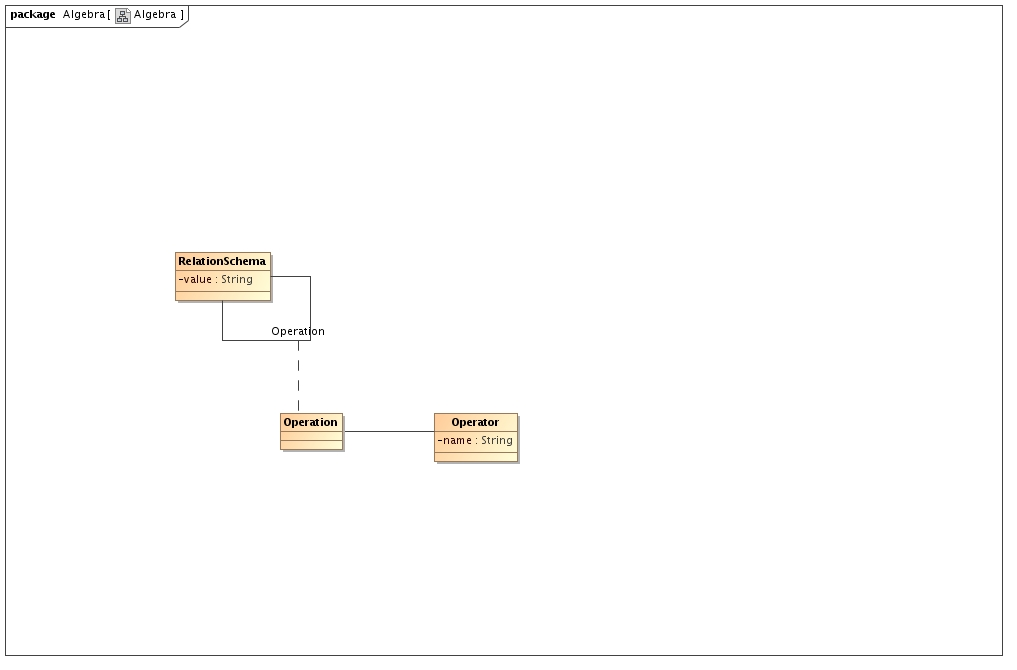
\includegraphics[width=220mm]{Algebra.jpg}

\end{document}
